\chapter{Ejecución del código}
\label{run1}
Aquí se presenta el archivo que genera el programa al correrlo, con algunas de las variables del mismo para permitir su seguimiento.

\section{Exponentes y Probabilidades} 
Aquí se muestra cómo el programa va calculando la matriz de probabilidades de transición, la que se espera que, con una buena cantidad de ejecuciones, converja hacia los valores de la ruta esperada.

En el ejemplo que sigue, solo se ejecutan 33 iteraciones para poder apreciar los valores intermedios que van resultando, pero esta puede crecer a más de mil iteraciones, si se quiere, aunque, como se ve en el análisis de la aplicación, se puede estimar la cantidad de iteraciones mínima que conviene ejecutar para alcanzar la convergencia.

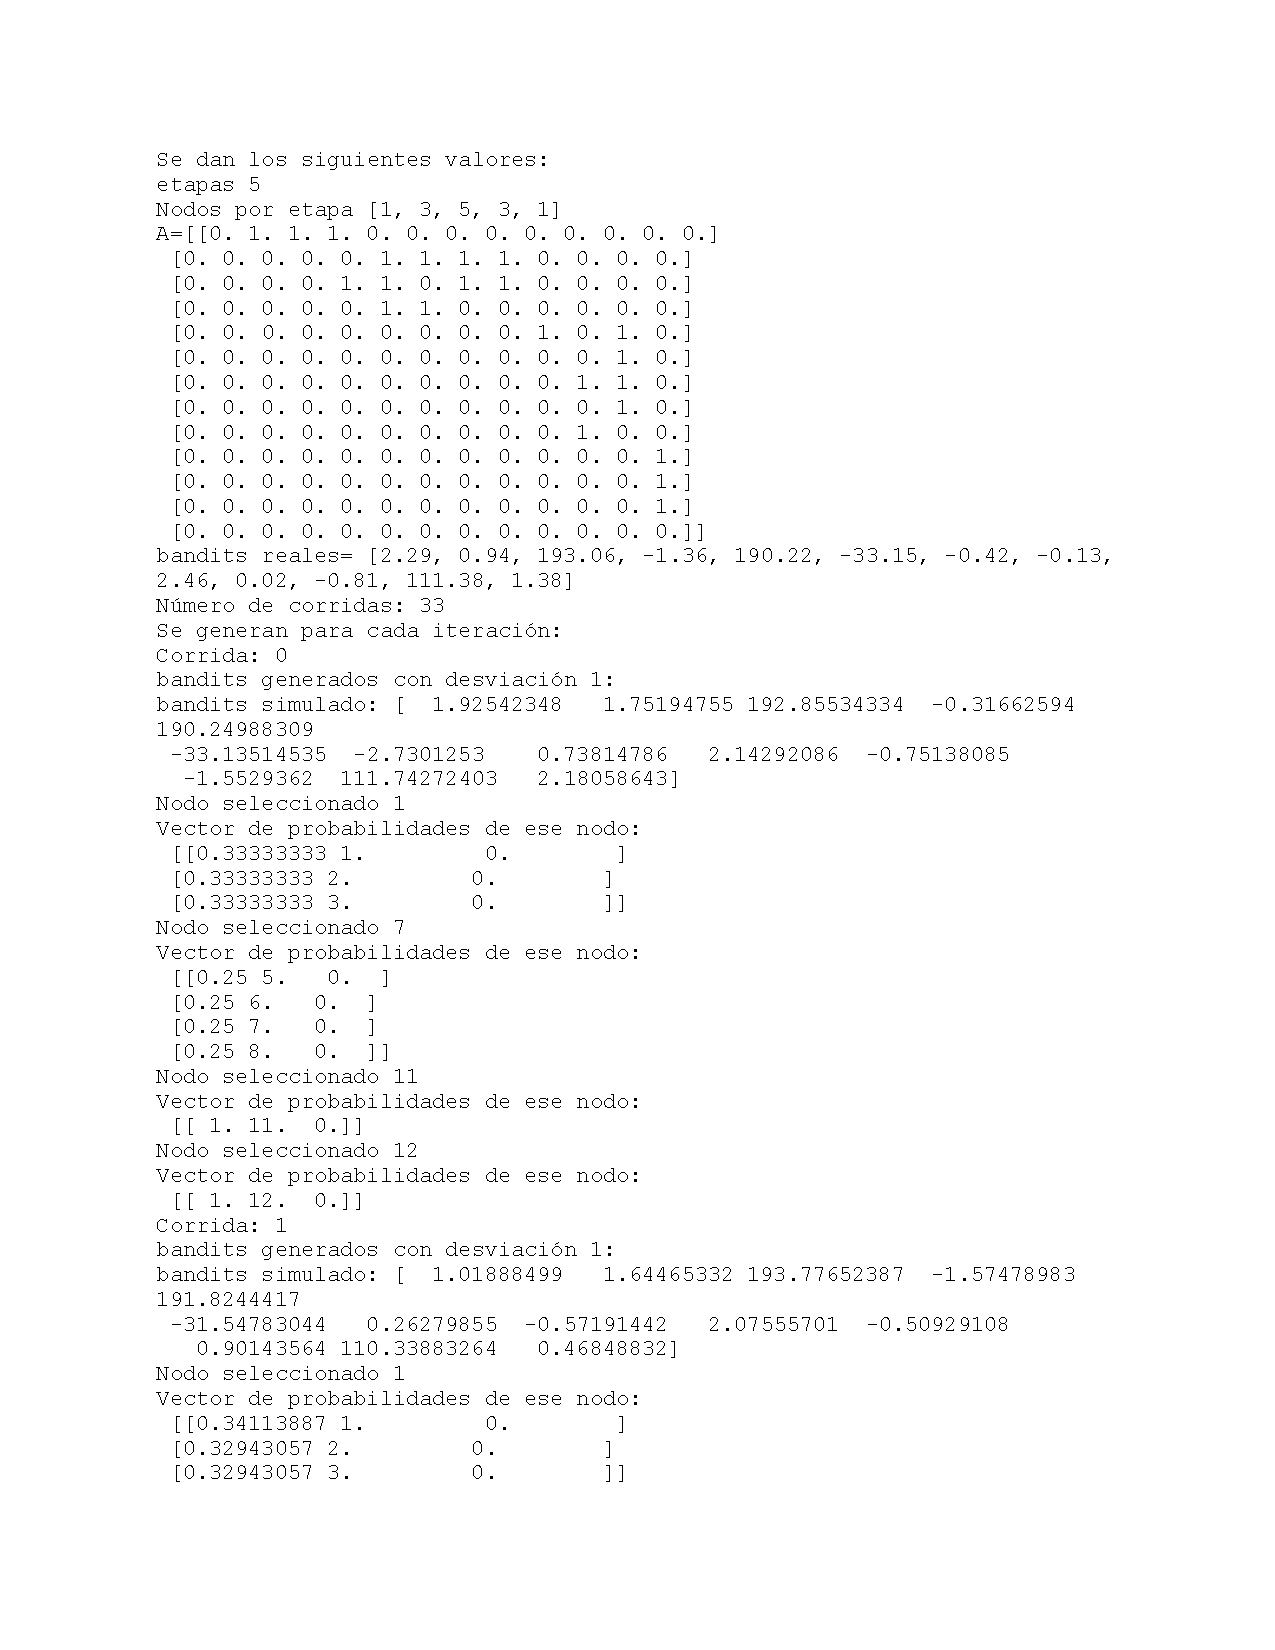
\includepdf[pages=-]{ResultPrib}

\section{Multiarmed-bandit} 
Con los mismos valores de nodos que se van calculando aprovechando las probabilidades generadas por la aplicación ya descrita, se hace aquí un cierre tradicional como lo haría el algoritmo Multiarmed-bandit, el cual va promediando las ganancias que van recibiendo cada una de las respuestas que históricamente se van generando en cada una de las iteraciones, y al final de esta da como respuesta la que tenga mejor ganancia promedio.
Se observa al final una comparación con la respuesta que aparece la mayor cantidad de veces, pero que, no necesariamente es la óptima, como se puede apreciar en sus ganancias.

Todo esto se puede corroborar en los resultados de las 33 rutas que se muestra con su respectivo paso a paso en que fueron generadas.

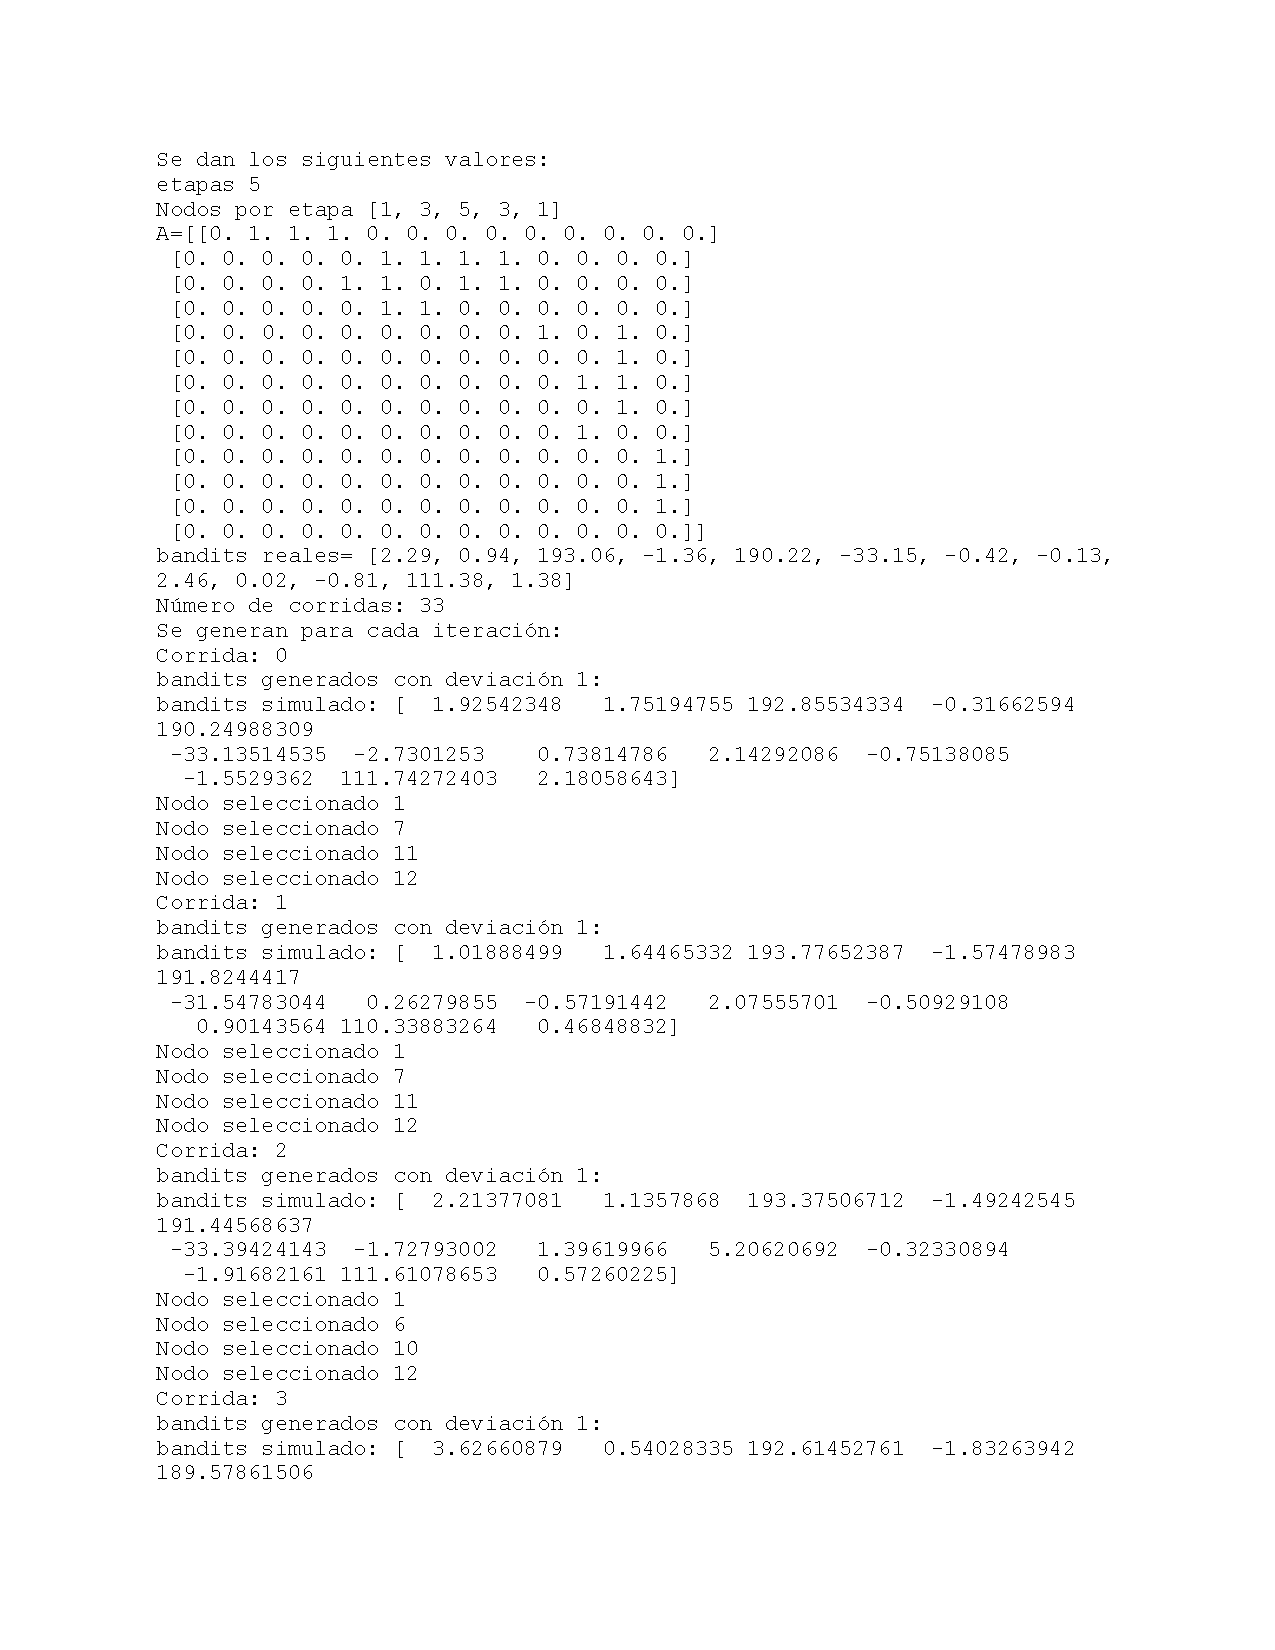
\includepdf[pages=-]{ResultBandit}
